\chapter{INTRODUCTION} \label{chap_introducao}

According to Moore's law \cite{Intel}, the number of transistors in an integrated circuit doubles every two years. Initially, Moore's law was merely an observation; over time, however, it became a goal for the electronics industry, as shown in Figure~\ref{fig:lei_de_moore}.

\begin{figure}[H]
\centering
\caption{Moore's law.}
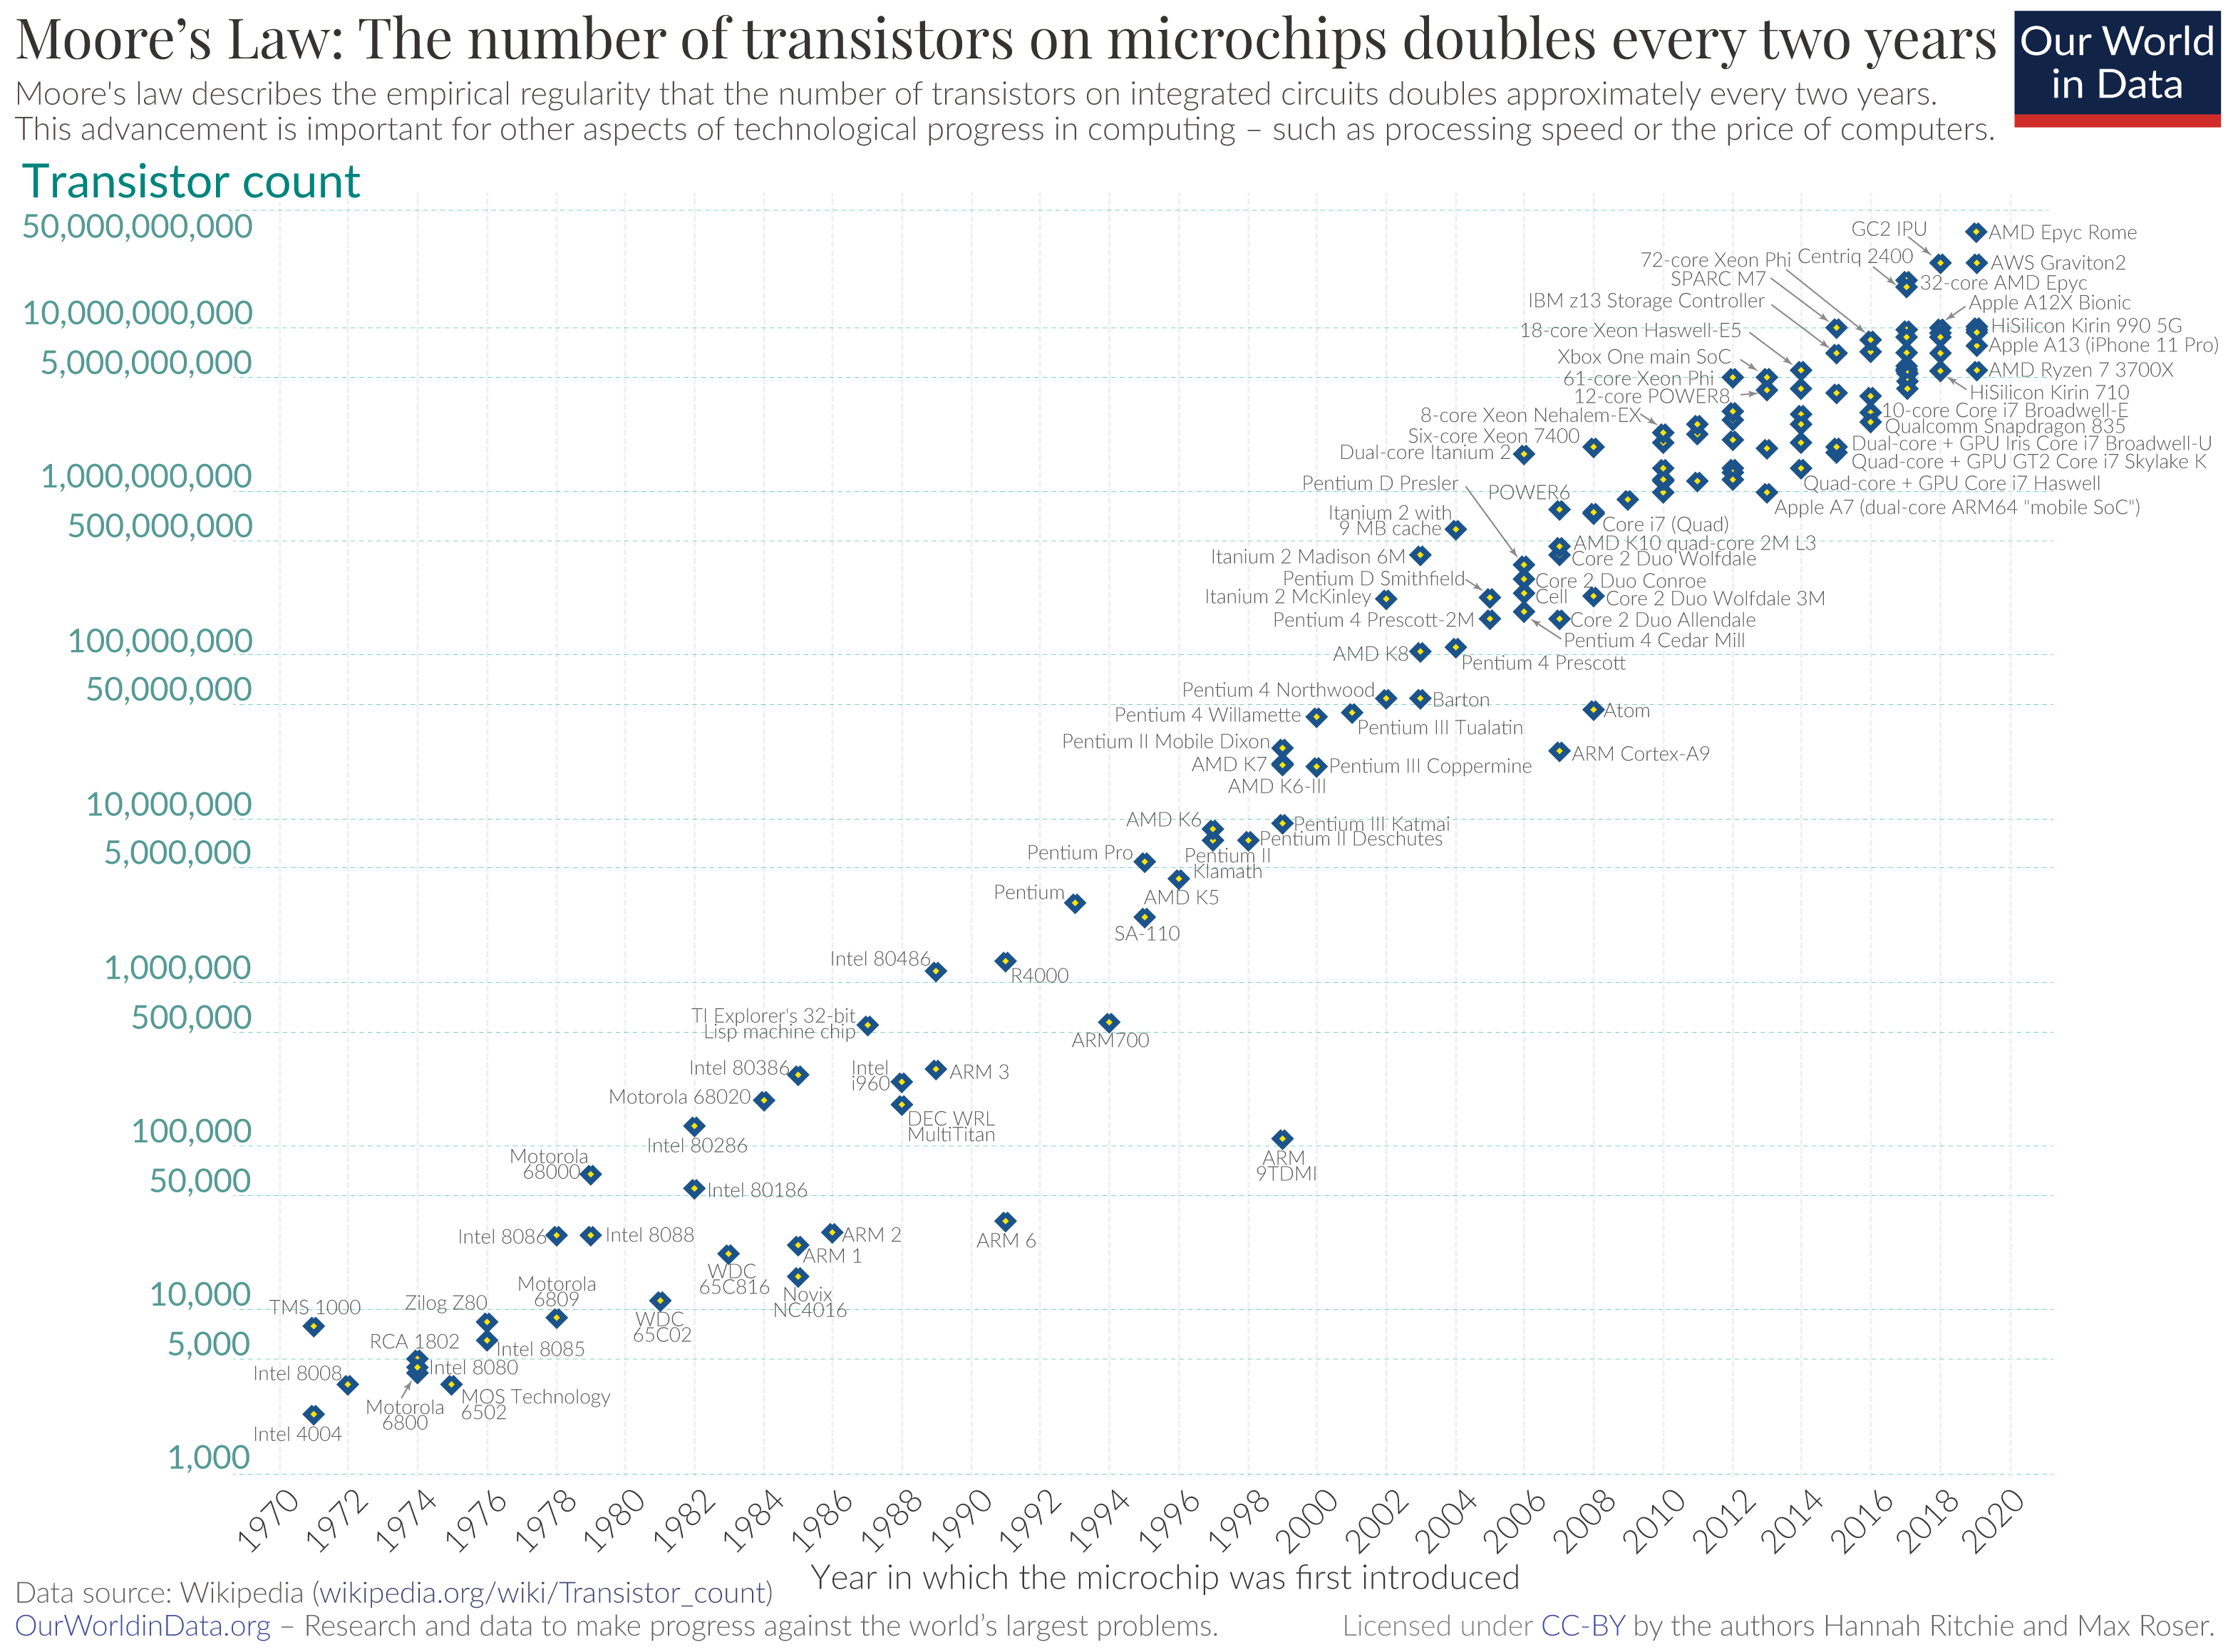
\includegraphics[width=\textwidth]{imagens/Moores_Law.png}
\smallcaption{Source: Our World in Data.}
\label{fig:lei_de_moore}
\end{figure}

With continued advances in the production of microchips and processors, transistors are approaching their minimum possible physical size, and the processing power of classical computers may therefore be approaching its limit \cite{Nielsen}. However, the complexity of computational problems tends to continue increasing. It may therefore become necessary to turn to a tool such as quantum computers, which may offer an advantage when solving certain problems considered difficult in classical computing \cite{Mermin2007QComputerScience, Wong2022IntroductionClassicalQuantum}.

Unlike classical computers, quantum computers are machines that use properties of quantum mechanics to perform their operations \cite{Wong2022IntroductionClassicalQuantum}. Whereas classical computers encode and process information stored in bits, quantum computers encode information in qubits (quantum bits), which allow states corresponding to superpositions of the classical states 0 and 1 \cite{Nielsen}. Nevertheless, current quantum machines still face significant limitations and challenges that affect their ability to perform machine learning tasks efficiently.

One of the main limitations of current quantum computers is noise. Qubits are susceptible to errors caused by several sources of noise, ranging from cosmic rays and interactions with neighboring qubits to thermal, electronic, and electromagnetic noise \cite{Nielsen}. These errors may lead to incorrect results and affect the accuracy of calculations performed by a quantum computer. Noise is a significant concern in quantum systems because of the sensitivity of qubits and the need to maintain quantum coherence during operations.

Another limitation of current quantum computers is the lack of standardization and stability. Different architectures and technologies are used to implement quantum computers, and no single standard has been widely adopted. This makes it difficult to reproduce results on different quantum machines and to compare their performance. In addition, quantum technologies are constantly evolving and new approaches are being explored, which hinders the stability and reliability of current quantum systems.

These limitations have significant implications for the use of quantum computers in machine learning tasks. Machine learning algorithms, such as those used for data classification, depend on accuracy and efficient processing to produce reliable results. Noise and the lack of standardization in quantum computers may adversely affect the performance of these algorithms, making them less effective than their classical counterparts.

In this context, several approaches to data classification on quantum computers use supervised machine learning models, including quantum support vector machines (QSVMs) \cite{Rebentrost2014QSVM}, quantum principal component analysis (qPCA) \cite{Lloyd2014qPCA}, and quantum neural networks (QNNs) \cite{Abhijith2022QuantumAlgorithm}, among others. This thesis, however, focuses on the variational quantum classifier \cite{Havlicek2019qSupervisedLearning}, which is built on the same quantum feature-space encoding.

\section{Objective} \label{sec1}

This thesis investigates the current performance of a quantum computer on the task of classifying data from the Iris dataset by comparing it with a classical classifier. The motivation for this study is to evaluate the capability of a real quantum computer on a machine learning problem, specifically in the area of data classification.

For this purpose, a supervised machine learning method, the quantum support vector machine, is adapted to run on a quantum computer. The Iris dataset was chosen as the case study because it is widely used in the scientific community as a benchmark for classification algorithms.

By comparing the classical classifier with a real quantum computer, this study seeks to obtain insights into the current performance of quantum computers on data classification tasks and to identify their limitations. This analysis contributes to advances in quantum computing and machine learning by providing important information about the possibilities and challenges involved in applying quantum methods in this domain.

Thus, this thesis contributes to the understanding of the current state of quantum computing in relation to machine learning and establishes a basis for future research and development in this constantly evolving area.

In summary, a variational quantum classifier \cite{Havlicek2019qSupervisedLearning} is applied to classify the Iris dataset. The classifier is constructed from quantum circuits that encode classical information into quantum states, as described in Section~\ref{Encoding}, and perform learning, as described in Section~\ref{ansatz}. The learning circuit has a predefined topology and a set of parameterized quantum gates. Training consists of learning the quantum-gate parameters that optimize the chosen cost function.

\section{Thesis Structure} \label{sec2}

This thesis is organized as follows. Chapter~\ref{chap_trabalhos_relacionados} presents the related work and the current state of the field. Chapter~\ref{chap:conceitos} details the quantum-physics concepts used in the study. Chapter~\ref{chap_metodologia} presents the methodology, including the programming language, techniques, and stages. Chapter~\ref{chap_resultados} discusses the project results. Finally, Chapter~\ref{chap_conclusao} presents the conclusions reached during the development of this work.